\chapter*{Blog}
        \addcontentsline{toc}{chapter}{Blog}
        \chaptermark{Blog}
	\markboth{Blog}{Blog}
	
	This is the portion of the thesis that I will update regularly with rough notes, lit reviews, results, etc. some of which will be worked in to the real document after some polishing. 
	\section{Goals}
	\begin{itemize}
	\item{10/14: Define specific problem.}
	\item{Fall Break: Experimental Setup}
	\item{Winter Break: Lit Review Complete}

	\end{itemize}

	
	
	\section{To Do}
	\begin{itemize}
	\item{Obtain flashdrives.    Miguel 9/30/14}
    \item{Learn Bohmian Mechanics. Miguel 11/4/14}
    \item{Find walking regime. Miguel 11/4/14}
    \item{Set up Accelerometer (should arrive around 11/19/14). Miguel 
 11/6/14}
     \item{Learn de Broglie's interpretation of QM. Miguel 11/6/14}
	\end{itemize}
	
	\subsection{Done}
	\begin{itemize}
	\item{Order Accelerometer.    Miguel 11/6/14}
	\item{Learn Basics of Bohmian Mechanics. Miguel 10/28/14}
	\item{Make tray. Miguel 10/20/14}
	\item{Sort out camera situation. Miguel 10/20/14}
	\item{Learn how to use the new \LaTeX\ and Github setup. Miguel 9/30/14}
	\end{itemize}
	
	\section{Literature Reviews}
	
(Important: Particle-wave association on a fluid interface (Protiere 2006)).

	    In this annual review, Bush describes some of the characteristics of the bouncing oil drop experiment that are analagous to effects witnessed in the quantum mechanical world (single-particle diffraction, tunneling, quantized orbits, orbital level splitting, and spin states). Dynamics of the walker are described mathematically. Finally, comparisons to de Broglie's orginal formulation of QM (and not Bohm's) and Stochastic Electrodynamics (?) are made. (Most coming from Pilot-Wave Hydrodynamics (Bush 2015))
	    \subsubsection{Basic Parameters}
	       Consider a fluid of density $\rho$, viscosity $\nu$, and surface tension $\sigma$, in a bath of depth $H$ driven vertically at an amplitude $A_0$ at frequency $f=\omega/{2\pi}$. By defining $\mathnormal{\gamma}=A_0\omega^2$, the effective gravity in the frame of reference of the bath is $g+\gamma~\mathrm{sin}(\omega t)$. The oil droplet of diameter $D$ bounces in the regime $\gamma<\gamma_F$, where $\gamma_F$ is the Faraday threshold (at this point, Fraday waves appear). The important experimental limits are outlined in \refTab{approxlimits}. 
	       \begin{table}[htdp] 
\caption[Basic Table 1]{Approximate Limits for Bouncing Drop Behavior} 
\begin{center} 
\begin{tabular}{c c c} 
\toprule 
  Parameter &  Lower Limit & Upper Limit \\
  \midrule
Viscocity $\nu$ (cSt) & 10 & 100 \\ 
Bath Depth $H$ (mm) & 4 & 10 \\
Frequency $f$ (Hz) & 20 & 150 \\
Amplitude $A_0$ (mm) & 0.1 & 1 \\
Drop Diameter $D$ (mm) & 0.6 & 1.0 \\
\bottomrule 
\end{tabular}
\end{center}
\label{approxlimits} 
\end{table}	

For certain parameters, the bouncing drop will behave differently. The vibration number describes ``the relative magnitude of the forcing frequency and the drop's natural oscillation frequency," and is given by:
	       	      
\begin{equation} \label{vibrationnumber}
V_i = \frac{\omega}{2}\sqrt{\frac{\rho D^3}{2\sigma}}
\end{equation}   	       	       
	       	       The natural frequency of the droplet occurs around $V_i = 0.65$, where the droplet can exhibit both walking and bouncing behaviors. Setting up a plot with $V_i$ on the y axis and (dimensionless) ${\gamma}/{g}$ on the x axis can help in showing the behavior of the droplet, shown in \refFig{regime}. 
	    
	    \begin{figure}[h]
	% the options are h = here, t = top, b = bottom, p = page of figures.
	% you can add an exclamation mark to make it try harder, and multiple
	% options if you have an order of preference, e.g.
	% \begin{figure}[h!tbp]
	   
	       \centering
	    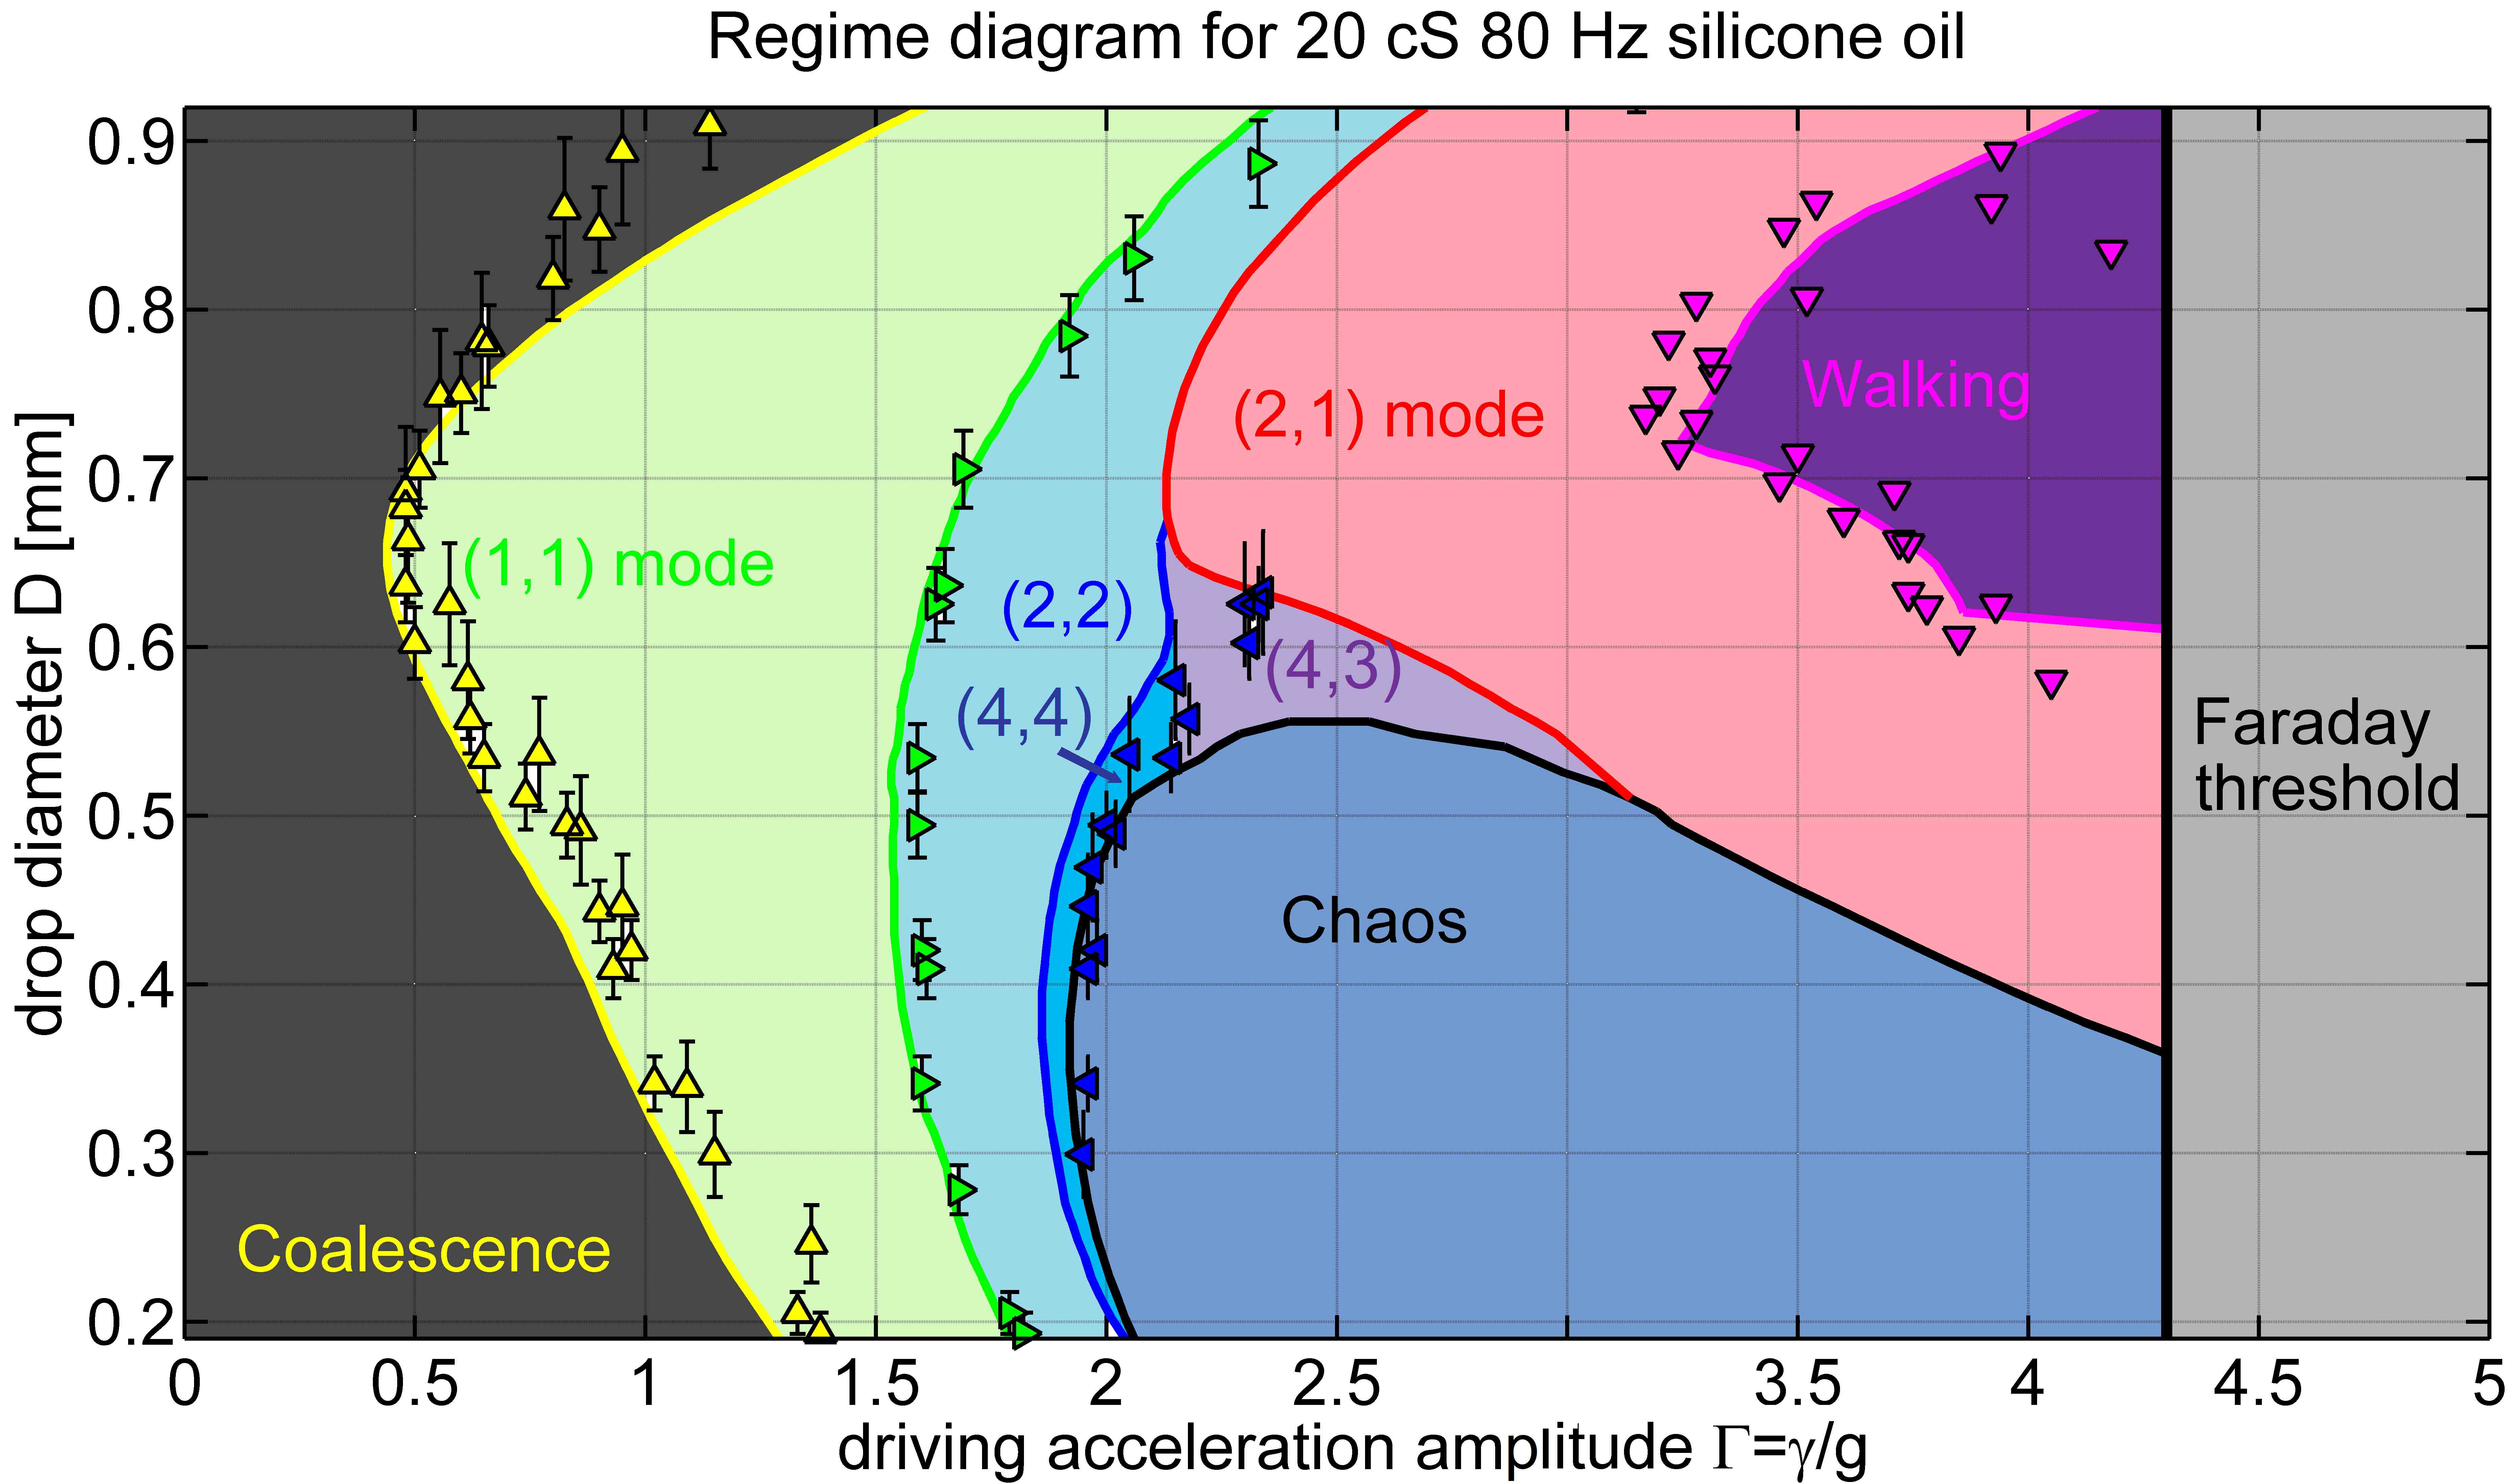
\includegraphics[scale=0.075]{Regime-Mega}
	     \caption{The different bouncing regimes for the oil drops of 20 cS silicon oil and at $f$ = $\omega / 2\pi$ = 80 Hz. The parameters ($m$,$n$) describe the droplet that bounces $n$ times in $m$ forcing periods. }
	 \label{regime}
	\end{figure}

The various modes seen in \refFig{regime} can be described by ($m$,$n$), where $n$ is the number to times the droplet contacts the surface over period $m/f$. For example, in the (1,1) mode, the droplet hits the oil bath once per driving period. In the (2,2) mode, the drop makes two bounces of differing heights. 
	       
            \subsection{Path Memory}
            Path memory is a parameter that can be varied in this setup. Every time the droplet impacts the bath, it creates a radial traveling wave. Over the course of many bounces, a wavefield composed of a superposition of the many waves arises. If the bouncing droplet impacts the wavefield in such a way that it recives a lateral force from the slope of the wave, then it will be pushed to the side slightly. The next time the droplet makes contanct with the bath, it will again be pushed to the side. This propels the bouncing droplet, causing it to walk across the surface of the bath. These ``walkers" are pushed in a direction dictated by previous impacts, and so it is said that the oil bath ``remembers" the previous bounce.	  
            
            Damping the waves results in a low-memory limit, since the walker is affected by only the previous impact. In an undamped system (approaching the Faraday threshold), the system becomes high-memory because walker can be affected by waves from many impacts ago. The quantum like features of this experiment arise in the high-memory limit. (For more, Eddi et. al, 2011b: Information stored in Faraday waves.) 

            \subsection{Single-Particle Diffraction}


\subsubsection{de Broglie vs. Bohm}
	       \subsection{Tunneling}
	       The guiding wave field can be partially reflected off of an edge or even a change in depth of the oil bath. This effect can be seen when a walker is pushed back from a under-the-surface step, seemingly without any contact. In rare cases, the walker will actually tunnel across the step; that is, it will continue to walk along the surface of the oil bath and pass over the step without reflection. In the first experiment done by Eddi et al., they demonstrated tunneling by by building square ``corrals" of varying thicknesses. In the second experiment, they built a rhombus shape which forced the walker across the center of a rhombus. The barrier was placed perpendicular to the direction of travel of the walker, so that it would hit the wall directly rather than at an angle (as in the square corral). ``The tunneling probability decreases exponentially with the barrier width and increases as the Faraday threshold is approached." Eddi et. al also found that the probability of tunneling increased with the velocity of the walker. (For more, Eddi et. al 2009b: Unpredictable Tunneling of a classical wave-particle association.)
	       
	       
	        The unpredictability of the tunneling comes from the complex interatction between the drop and its guiding wave. 

\subsection{Motion in a Confined Geormetry}
By tracking the droplet as it bounces around the tray over a period of time, one can look at the overall statistical behavior of the droplet. Two experiments tracked walkers in an experimental coral (Harris and Bush, 2013, Harris et al. 2013) in the high-memory, chaotic motion regime. A histogram of the statistical data shows that the "probability of finding a walker at a given point in the corral is roughly prescribed by the amplitude of the Faraday wave mode of the cavity at the prescribed forcing frequency."

Quantum corral experiments performed by Crommie et al. (Crommie et al. 1993 a b) present similar findings. In the experiment, electrons were confined in a Cu(III) substrate using barriers of iron adatoms. Using tunneling spectroscopy, the electrons were found to have a specific resonances depending on the corral shape. As in the case of Harris' circular corral experiment where the corral and the Faraday wavelength, $\lambda_F$, dictate the wavelike statistical patter, in the quantum experiment the corral and the \textit{de Broglie} wavelength, $\lambda_{dB}$, dictate the form of the wavelike statistical pattern. 

\subsection{Bouncing Mechanics}
In the regime of walkers we have $R_e \sim 20$, $B_0 \sim 0.1$, and $W_e \sim 0.1$. For the millimeric walkers, the dominant force comes from impact of the curvature of the surface. Gilet and Bush (2009: Chaotic bouncing of a drop on a soap film, and the fluid trampline: droplets bouncing on a soap film) show that the surface of the vibrating oil can be modeled with a soap film, where the soap film acts like a linear spring. 

As the oil bath is forced up and down, a tiny droplet of oil will ``walk" across the surface. Mol\'{a}\v{c}ek and Bush have developed an equation of a droplet that describes the trajectory of the walking droplet, ignoring the verical dynamics by time averaging them out (cite: J. Mol\'{a}\v{c}ek and J. W. M. Bush, ``Drops walking on a vibrating bath: towards a hydrodynamic pilot-wave theory" J. FluidMech. 727, 612-647 (2013).). The trajectory of the walking droplet of mass $m$ at position $\textbf{x}(t) = (x(t),y(t))$ is given by
\begin{equation}
m \ddot{\textbf{x}} + D \dot{\textbf{x}} = -mg\nabla h(\textbf{x},t) 
\end{equation}
where $D$ describes the drag coefficient and $h(\textbf{x},t)$ describes the shape of the wavefield. Thus the second term describes the time averaged drag from both the flight and the impact of the droplet (as usual, depends on the velocity), and the third term describes the propulsive wave force resulting from drops landing on the inclined wave surface. 

The wavefield is quite complicated because it depends on the memory. For a single impact of a droplet, Oza et al. argue the surface wave can be approximated with an integral of a monochromatic radial Bessel function of the first kind

\begin{equation}
h(\textbf{x},t) = \frac{F}{T_F} \int_{-\infty}^{t} J_0 \frac{(k_F |\textbf{x}(t)-\textbf{x}(s)|)}{|\textbf{x}(t)-\textbf{x}(s)|} (\textbf{x}(t)-\textbf{x}(s))e^{-(t-s)/(T_F M_e)} ds
\end{equation}
with $F$ giving the wave force coefficient (estimated in the above source), $T_F$ describing the Faraday period, and $k_F$ describing the Faraday wave number determined by the Faraday wavelength $\lambda_F = 2π/k_F$ (integral from A. U. Oza, D. M. Harris, R. R. Rosales, and J. W. M. Bush, "Pilot-wave dynamics in a rotating frame: on the emergence of orbital quantization" J. Fluid Mech. 744, 404-429 (2014).). (Faraday was a popular guy.) Finally, that last term $M_e$ is the nondimensional memory parameter $M_e = T_d/[T_F(1-\gamma / \gamma_F)]$ (with $T_d$ being the unforced decay time).

\section{Experimental Setup}

\section{Bohmian Mechanics}

\subsection{Formalism}
\subsubsection{The Schroedinger Equation and $\psi$}

We begin with the Schoedinger equation

\begin{equation}
i \hbar \frac{\partial}{\partial t}\psi = \hat H \psi
\end{equation}
where $\hat H$ is the Hamiltonian and $\psi$ is the wavefunction. The Hamiltonian can be expanded (assuming there is no electric field) to give

\begin{equation}
\label{SE}
i\hbar\frac{\partial}{\partial t} \psi(\mathbf{x},t) = \left [ \frac{-\hbar^2}{2 m}\nabla^2 + V(\mathbf{x},t)\right ] \psi(\mathbf{x},t)
\end{equation}
where $V(\mathbf{x},t)$ is the potential energy of the system. The solution $\psi$ is of the form:

\begin{equation}
\psi(\mathbf{x},t) = R(\mathbf{x},t) e^{i S(\mathbf{x},t) / \hbar}
\end{equation}
where $S$ and $R$ are real. Plugging in our equation for $\psi$ into the Schoedinger equation (\refeq{SE}) will produce two separate equations: one giving the time derivative of $R$ and the second giving the time derivative of $S$. From these equations, a Hamilton-Jacobi equation can be written for a quantum system.
    Let's begin by computing the left hand side of \refeq{SE} in terms of $R$ and $S$.   

$$
\begin{align*}
i\hbar\frac{\partial}{\partial t} \psi(\mathbf{x},t) &= i \hbar\left(\frac{\partial R}{\partial t} e^{i S / \hbar} + R \frac{i}{\hbar}\frac{\partial S}{\partial t} e^{i S / \hbar}\right)
\\ &= i \hbar \left(\frac{1}{R} \frac{\partial R}{\partial t} + \frac{i}{\hbar}\frac{\partial S}{\partial t}\right) \psi(\mathbf{x},t) 
\\ &= \left(i \hbar \frac{1}{R} \frac{\partial R}{\partial t} - \frac{\partial S}{\partial t}\right) \psi(\mathbf{x},t)
\end{align*}
$$
Let's leave that alone for a little bit, while we focus on the right hand side of \refeq{SE}. Since it's a little more complicated, we will start with one term of the right hand side:

$$
\begin{align*}
\nabla^2 \psi(\mathbf{x},t)  &= e^{i S / \hbar} \nabla^2 R + \left(\frac{i}{\hbar}\right)^2 (\nabla S)^2 R e^{i S / \hbar} + \left(\frac{i}{\hbar}\right) R e^{i S / \hbar} (\nabla^2 S) + \left(\frac{2i}{\hbar}\right) (\nabla R \cdot \nabla S) R e^{i S / \hbar}
\\ &= \left(\frac{\nabla^2 R}{R} - \left(\frac{\nabla S}{\hbar}\right)^2  + \left(\frac{i \nabla^2 S}{\hbar}\right) + 2 i \left(\frac{\nabla R \cdot \nabla S}{\hbar}\right) \right) \psi(\mathbf{x},t) 
\end{align*}
$$

Now the hard part is done, and we can say that the right hand side of \refeq{SE} is given by 

$$
\begin{align*} 
\left [ \frac{-\hbar^2}{2 m}\nabla^2 + V(\mathbf{x},t)\right ]\psi(\mathbf{x},t) &= \left [-\frac{\hbar^2  \nabla^2 R}{2 m R} + \left(\frac{(\nabla S)^2}{2 m}\right)  - i \hbar \left(\frac{\nabla^2 S}{2 m}\right) - i \hbar \left(\frac{\nabla R \cdot \nabla S}{m}\right) + V(\mathbf{x},t) \right]\psi(\mathbf{x},t) 
\end{align*}
$$

Ok, now that we've got that done, the next part will be super easy. Starting with Schrodinger's equation and plugging in left and right hand sides we calulated seperately. 

$$
i\hbar\frac{\partial}{\partial t} \psi(\mathbf{x},t) = \left [ \frac{-\hbar^2}{2 m}\nabla^2 + V(\mathbf{x},t)\right ] \psi(\mathbf{x},t)
$$
$$
\left(i \hbar \frac{1}{R} \frac{\partial R}{\partial t} - \frac{\partial S}{\partial t}\right) \psi(\mathbf{x},t) =\left [-\frac{\hbar^2  \nabla^2 R}{2 m R} + \left(\frac{(\nabla S)^2}{2 m}\right)  - i \hbar \left(\frac{\nabla^2 S}{2 m}\right) - i \hbar \left(\frac{\nabla R \cdot \nabla S}{m}\right) + V(\mathbf{x},t) \right]\psi(\mathbf{x},t) 
$$
Now we can divide out $\psi$ from both sides
$$ 
i \hbar \frac{1}{R} \frac{\partial R}{\partial t} - \frac{\partial S}{\partial t} = -\frac{\hbar^2  \nabla^2 R}{2 m R} + \left(\frac{(\nabla S)^2}{2 m}\right)  - i \hbar \left(\frac{\nabla^2 S}{2 m}\right) - i \hbar \left(\frac{\nabla R \cdot \nabla S}{m}\right) + V(\mathbf{x},t)
$$
and group the imaginary numbers on the left side and the real numbers on the right side 
$$ i \hbar \frac{1}{R} \frac{\partial R}{\partial t} + i \hbar \left(\frac{\nabla^2 S}{2 m}\right) + i \hbar \left(\frac{\nabla R \cdot \nabla S}{m}\right) = \frac{\partial S}{\partial t} -\frac{\hbar^2  \nabla^2 R}{2 m R} + \left(\frac{(\nabla S)^2}{2 m}\right)  + V(\mathbf{x},t)
$$
Recall that both $S$ and $R$ are real. Note that the only way for all of the imaginary terms to equal all of the real terms is if they both equaled zero.
$$i \hbar \left(\frac{1}{R} \frac{\partial R}{\partial t} + \frac{\nabla^2 S}{2 m} + \frac{\nabla R \cdot \nabla S}{m}\right) = \left(\frac{\partial S}{\partial t} -\frac{\hbar^2}{2m}\frac{\nabla^2 R}{R} + \frac{(\nabla S)^2}{2 m}  + V(\mathbf{x},t) \right) = 0
$$
This then gives us two sepeate equations, one for the time derivative of $R$ and another for the time derivative of $S$.

\begin{equation}
\label{dR/dt}
\frac{\partial R}{\partial t} = -\frac{R}{2 m}\left(\frac{\nabla^2 S}{m}-2\nabla R \cdot \nabla S\right)
\end{equation}


\begin{equation}
\label{dS/dt}
\frac{\partial S}{\partial t} = \frac{\hbar^2}{2m}\frac{\nabla^2 R}{R} - \frac{(\nabla S)^2}{2 m} - V(\mathbf{x},t)
\end{equation}

What does this do for us? Both equations will provide helpful descriptions of our system.

\subsubsection{The Quantum Potential}

We can rewrite \refeq{dS/dt} in a provokative way 

\begin{equation}
\label{BohmHamiltonian}
- \frac{\partial S}{\partial t} = \frac{(\nabla S)^2}{2 m} + V(\mathbf{x},t) + \frac{\hbar^2}{2m}\frac{\nabla^2 R}{R}
\end{equation}
which should look suspiciously familiar. If I were to tell you that $\nabla S$ had units of momentum and $\partial S/\partial t$ units of energy, then this equation would look a lot like a Hamiltonian! The first term takes care of the kinetic energy, the second is the potential energy term, but we have this mysterious third term which we haven't ever encountered in classical mechanics. If we define this term as our ''quantum potential" 

\begin{equation}
\label{QuantumPotential}
U(\mathbf{x}) =  \frac{\hbar^2}{2m}\frac{\nabla^2 R}{R} = \frac{\hbar^2}{4m}\left[\frac{1}{2} \frac{\nabla^2 P}{P} - \frac{(\nabla P)^2}{P^2}\right] 
\end{equation}
then we really \textit{can} think of \refeq{BohmHamiltonian} as a Hamiltonian with an extra potential term thrown in to make it "quantum." Note that in cases where $\hbar$ is much smaller than the rest of the terms (i.e. not the quantum realm), then this quantum potential term goes away, and we are left with the regular Hamilton equation from classical mechanics. 

Recall that when writing a Hamiltonian, the potential terms govern the forces on the particle. For a conservative system, the force is given by F(x) = -$\partial U/\partial x$. If we include a quantum mechanical potential in our Hamiltonian, then this potential must cause a force on the paticle in addition to the one supplied by the $V(x)$ term. 


\subsubsection{Continuity Equation}
Plugging in the probability density $P(\mathbf{x},t) = R^2(\mathbf{x},t)$ into \refeq{dR/dt} also gives us something quite interesting.

MATH?

which we can finally express as 

\begin{equation}
\label{ProbCurrent}
\frac{\partial P}{\partial t} + \nabla \cdot \left( P \frac{\nabla S}{m} \right)
\end{equation}

In describing the quantum potential term it was mentioned that $\nabla S$ can be thought of as momentum, so then from our classical relationship between momentum and velocity  $\textbf{v}(\textbf{x},t)=\nabla S/m$ can be thought of as velocity. Then by defining the probability current as $j(\mathbf{x},t) = P\nabla S/m$ then we recover

\begin{equation}
\label{ProbCurrent}
\frac{\partial P}{\partial t} + \nabla \cdot j(\mathbf{x},t)
\end{equation}
known as the continuity equation! This tells us that $P$ is conserved over time.

\subsubsection{Finding $R$ and $S$}

